\documentclass[a4paper,
               % boxit,        % check whether paper is inside correct margins
               biblatex,       % biblatex is used
               keeplastbox,    % flushend option: not to un-indent last line in References
               % nospread,     % flushend option: do not fill with whitespace to balance columns
               % hyphens,      % allow \url to hyphenate at "-" (hyphens)
               % xetex,        % use XeLaTeX to process the file
               % luatex,       % use LuaLaTeX to process the file
               ]{jacow-2_1}    % uses jacow-2_1 to better support BibLaTeX
               
%
% CHANGE SEQUENCE OF GRAPHICS EXTENSION TO BE EMBEDDED
% ----------------------------------------------------
% test for XeTeX where the sequence is by default eps-> pdf, jpg, png, pdf, ...
%    and the JACoW template provides JACpic2v3.eps and JACpic2v3.jpg which
%    might generates errors, therefore PNG and JPG first
%
\makeatletter%
	\ifboolexpr{bool{xetex}}
	 {\renewcommand{\Gin@extensions}{.pdf,%
	                    .png,.jpg,.bmp,.pict,.tif,.psd,.mac,.sga,.tga,.gif,%
	                    .eps,.ps,%
	                    }}{}
\makeatother

% CHECK FOR XeTeX/LuaTeX BEFORE DEFINING AN INPUT ENCODING
% --------------------------------------------------------
%   utf8  is default for XeTeX/LuaTeX 
%   utf8  in LaTeX only realises a small portion of codes
%
\ifboolexpr{bool{xetex} or bool{luatex}} % test for XeTeX/LuaTeX
 {}                                      % input encoding is utf8 by default
 {\usepackage[utf8]{inputenc}}           % switch to utf8

\usepackage[USenglish]{babel}			 

\usepackage[final]{pdfpages}
\usepackage{multirow}
\usepackage{ragged2e}
 
\addbibresource{FRAPL01.bib}

%
% command for typesetting a \section like word
%
\newcommand\SEC[1]{\textbf{\uppercase{#1}}}

%%
%%   Lengths for the spaces in the title
%%   \setlength\titleblockstartskip{..}  %before title, default 3pt
%%   \setlength\titleblockmiddleskip{..} %between title + author, default 1em
%%   \setlength\titleblockendskip{..}    %afterauthor, default 1em

%\copyrightspace %default 1cm. arbitrary size with e.g. \copyrightspace[2cm]

% testing to fill the copyright space
%\usepackage{eso-pic}
%\AddToShipoutPictureFG*{\AtTextLowerLeft{\textcolor{red}{COPYRIGHTSPACE}}}


\begin{document}

\title{Status of the Square Kilometre Array}

\author{
	J. Santander-Vela\thanks{j.santander-vela@skatelescope.org},
	Lorenzo Pivetta, Nick Rees,\\
	representing the SKA Organisation, Macclesfield, United Kingdom
}
	
\maketitle

%2345678901234567890123456789012345678901234567890123456789012345678901-
\begin{abstract}
	The Square Kilometre Array (SKA) is a international project to build a number of multi-purpose radio telescopes, operating as a single observatory, that will play a major role in answering key questions in modern astrophysics and cosmology. It will be one of a small number of cornerstone observatories around the world that will provide astrophysicists and cosmologists with a transformational view of the Universe. Two major goals of the SKA is to study the history and role of neutral Hydrogen in the Universe from the dark ages to the present-day, and to employ pulsars as probes of fundamental physics. Since 2008, the global radio astronomy community has been engaged in the development of the SKA and is now nearing the end of the \emph{Pre-Construction} phase. This talk provides an overview of the current status of the SKA and the plans for construction, focusing on the computing and software aspects of the project.
\end{abstract}


\section{Introduction} % (fold)
\label{sec:introduction}
The Square Kilometre Array (SKA) is an international project that has the aim of building multi-purposes radio telescopes, with an equivalent collecting area of at least one square kilometre, and thus unprecedented sensitivity, so that key questions in modern astrophysics and cosmology can be answered.

The original SKA Science book was published in 2004~\cite{2004NewAR..48..979C}. In 2015, \citetitle{2015aska.confE.....}~\cite{2015aska.confE.....} was published with an update to the SKA science book after a decade of development of the SKA concept, incorporating more than 130 scientific use cases that will be possible thanks to the SKA telescopes.

Those science cases cover Galaxy Evolution, Cosmology and Dark Energy\footnote{http://skatelescope.org/galaxyevolution/}~\cite{2015aska.confE..67P, 2015aska.confE..16M, 2015aska.confE..51F}, Strong-Field Tests of Gravity\footnote{http://skatelescope.org/gravity-einstein-pulsars/}~\cite{2015aska.confE..36K}, Cosmic Magnetism\footnote{http://skatelescope.org/magnetism/}~\cite{2015aska.confE..92J}, The Cosmic Dawn and the Epoch of Reionisation\footnote{http://skatelescope.org/cosmicdawn/} ~\cite{2015aska.confE...1K}, and research on the Cradle of Life\footnote{http://skatelescope.org/cradle-life/}~\cite{2015aska.confE.115H}. The amount of physical disciplines foreseen to be encompassed by the SKA telescopes is one of the largest for any ground based facility to date.

The SKA project is currently in what is known as SKA Phase 1, or SKA1, in which two telescopes approximately with 10\% of the target collecting area are being built, namely SKA1-Mid, and SKA1-Low, in order to prove the feasibility of the techniques and derisk the construction of the next phase of the project, SKA Phase 2, or SKA2.

The goal is to have a single observatory entity, that will construct and operate two SKA1 telescopes (SKA1-Mid and SKA1-Low), with presence in three sites: Australia (SKA1-Low), South Africa (SKA1-Mid), and United Kingdom (Headquarters and central operations).

This talk focuses on the progress and status of the SKA1 telescopes. It starts by describing the SKA Organisation itself (Sec.~\ref{sec:ska_organisation}), and the SKA telescopes being designed (Sec.~\ref{sec:ska1_telescopes}). We continue with details on the Pre-Construction phase (Sec.~\ref{sec:ska1_preconstruction}), the challenging Data Flow and Processing (Sec.~\ref{sec:ska1_data_flow_and_processing}), and the Software and control challenges (Sec.~\ref{sec:ska1_software_control_system_guidelines_SAFe}). We summarise the main results in the Conclusions(Sec.~\ref{sec:conclusion}). 

% section introduction (end)

\section{SKA Organisation} % (fold)
\label{sec:ska_organisation}
The organisation overseing the SKA1 project is the SKA Organisation (SKAO), currently a limited liability non-for-profit company registered in England and Wales.

The SKAO is in the process of the becoming an Inter-Govermental treaty Organisation (IGO), not unlike the European Council for Nuclear Research (CERN), the European Molecular Biology Laboratory (EMBL), or the European Southern Observatory (ESO). The timeline for that process, and for the main design milestones, is detailed in Sec.~\ref{sec:ska1_preconstruction}.

Currently\footnote{https://skatelescope.org/participating-countries/} there are ten countries that are Full Members of the SKAO (listed in alfabetical order): Australia, Canada, China, India, Italy, New Zealand, South Africa, Sweden, The Netherlands, and United Kingdom. Other countries are involved in the design of the SKA1 telescopes, and it is estimated that \~20 countries and more than 100 organisations are contributed to that effort.

SKAO's headquartes are located within the boundaries of the Jodrell Bank Observatory, in the middle of the Cheshire plain.

As part of the UK commitment as host country for the SKAO HQ, and the IGO, an expansion to the HQ is being constructed with the intention of becoming a nexus for radio astronomy. The current status of the work, as of September 2017, can be seen in Fig.~\ref{fig:SKA-HQ2-aerial}.

\begin{figure}[!tb]
  \centering
    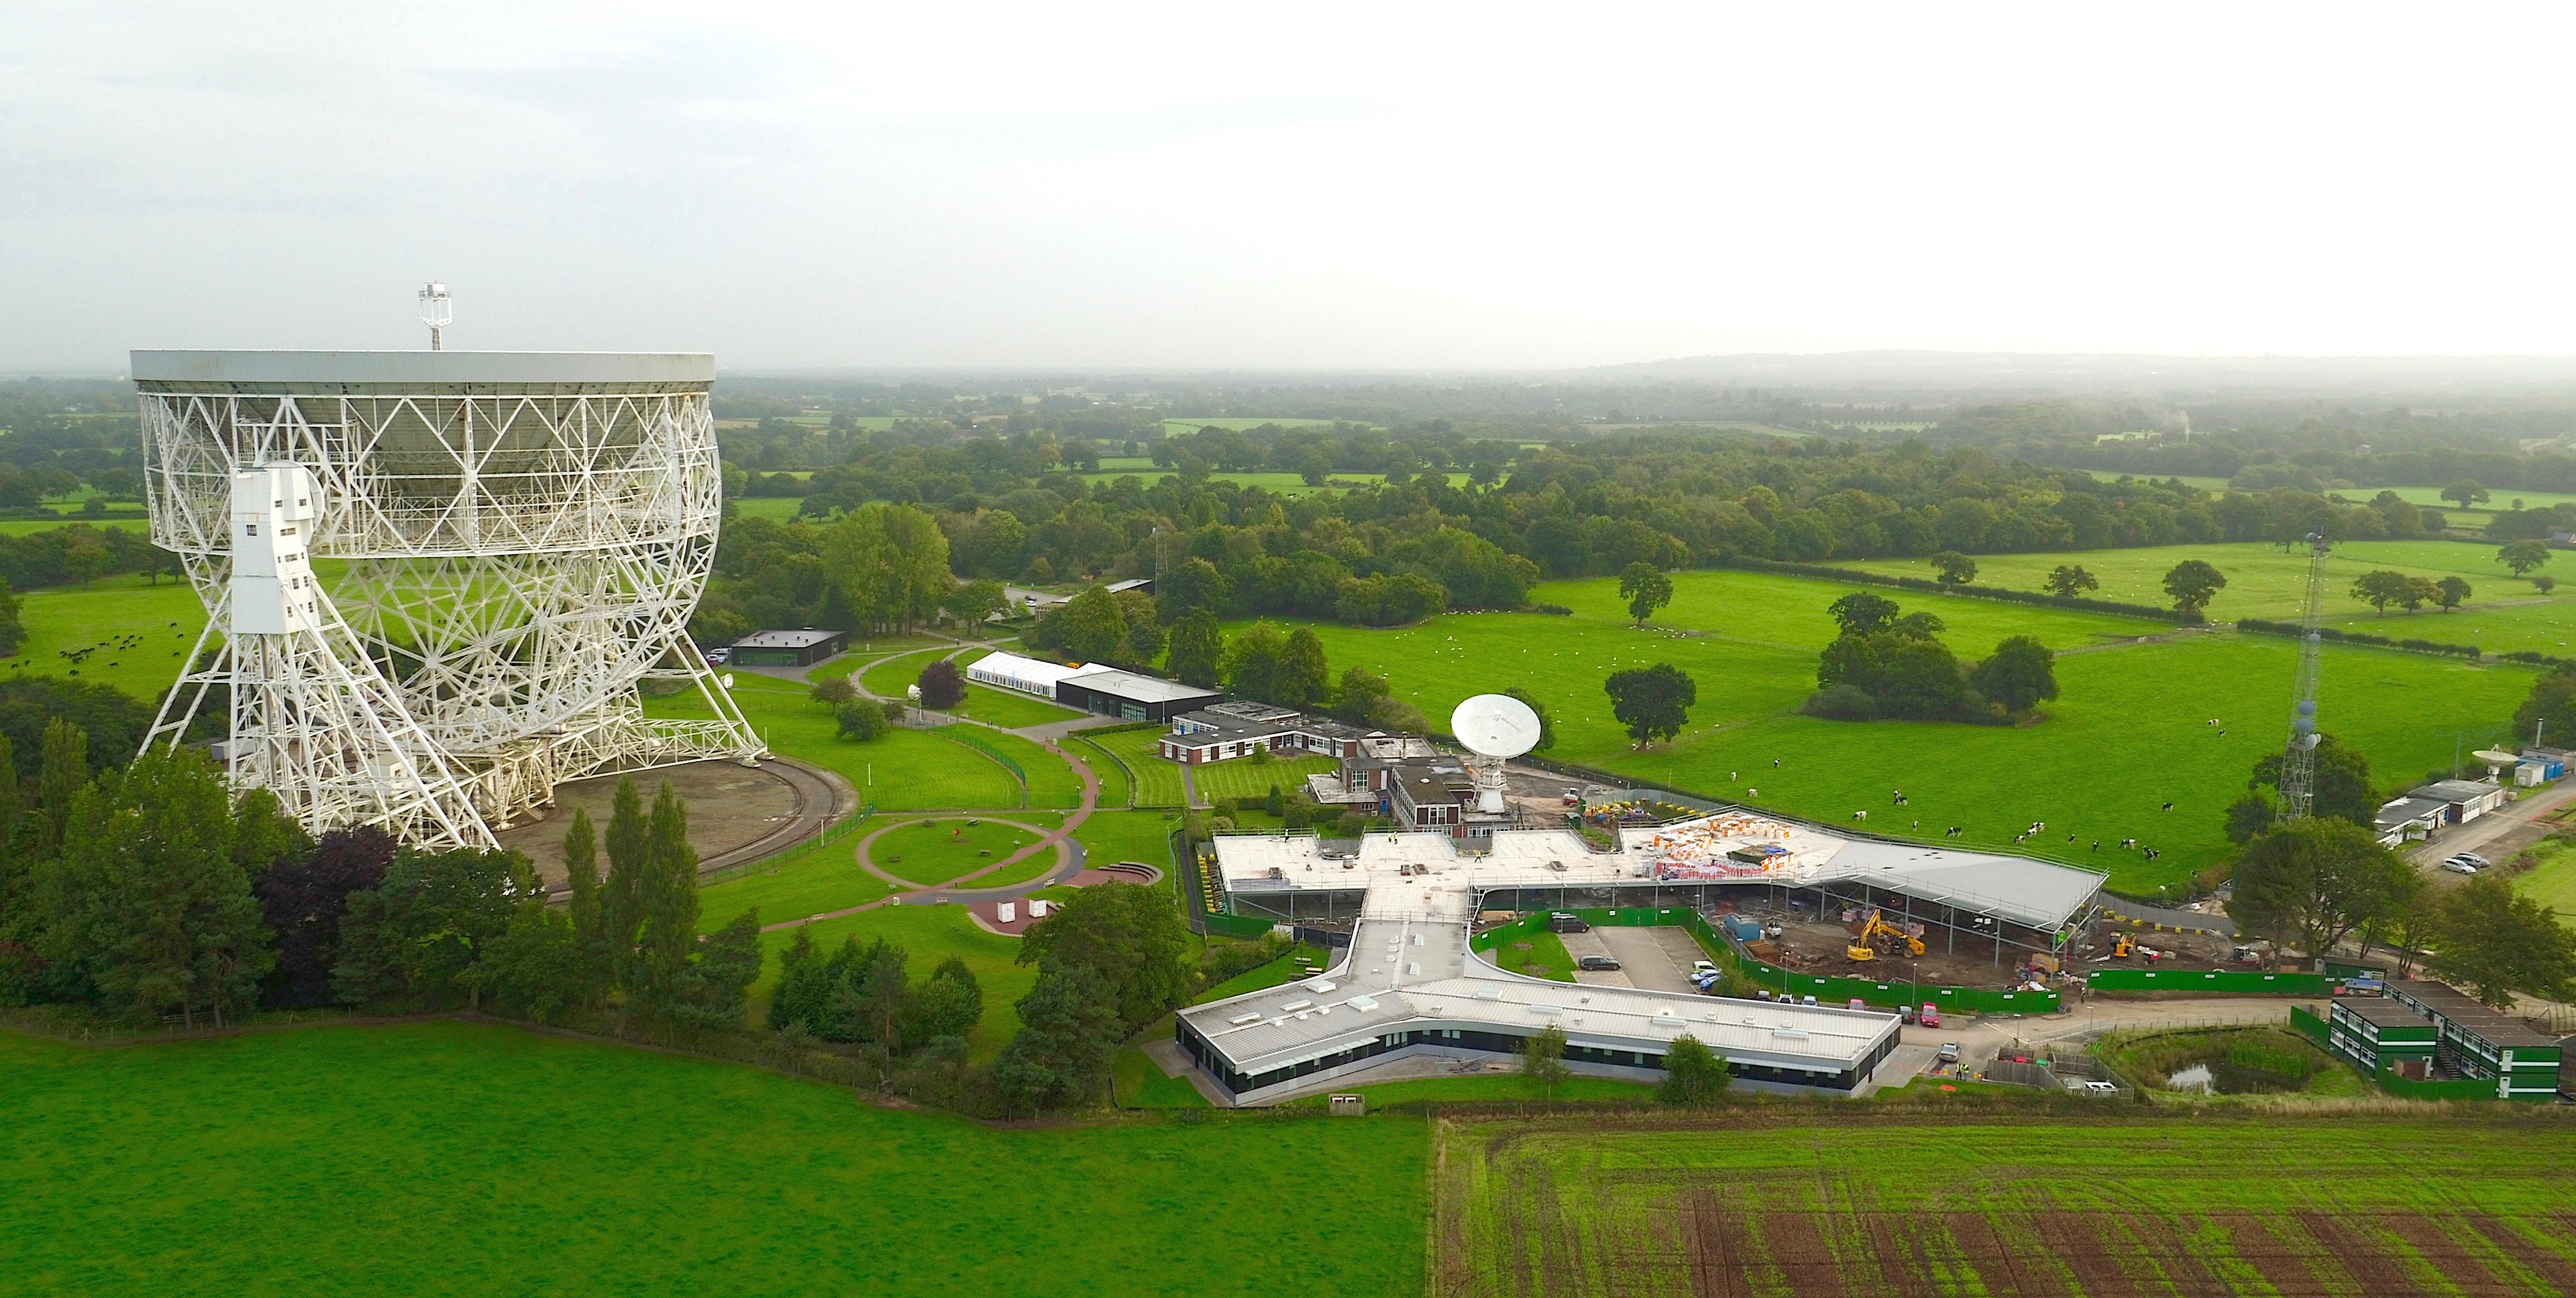
\includegraphics[width=\columnwidth]{FRAPL01f1}
  \caption{Aerial view of the current status of the SKAO HQ2 building, after the steel structure has been erected, and concrete slabs installed. The current SKAO HQ is in the foreground, Council chamber can be seen raising to the right.}
  \label{fig:SKA-HQ2-aerial}
\end{figure}

% section ska_organisation (end)

\section{SKA1 Telescopes} % (fold)
\label{sec:ska1_telescopes}

As previously indicated, in this Phase 1 (SKA1) we intend to build two telescopes, SKA1-Mid, and SKA1-Low, within a cost cap for both telescopes of 674~MEur (2016 value).

The SKA1-Low will be located in Western Australia, within the Murchison Radio-astronomy Observatory (MRO), which defines a Radio Quiet Zone for the benefit of the SKA1-Low, but also the Australian SKA Pathfinder (ASKAP) and Murchison Widefield Array (MWA) precursor telescopes. Fig.~\ref{fig:SKA1-Low_locations} shows where the MRO is located, together with the positions of Geraldton (the designated Engineering Operations Centre), and of the Pawsey Supercomputing Centre, currently the designated host for the Science Processing Facility.

\begin{figure}[!tb]
  \centering
    \includegraphics[width=\columnwidth]{FRAPL01f2}
  \caption{Relevant locations of SKA1-Low in Western Australia. The image shows the location of the Murchison Radio-astronomy Observatory,  the Engineering Operations Centre in Geraldton, and the Pawsey Supercomputing Centre, where we expect the Science Data Processor for SKA1-Low to be located.}
  \label{fig:SKA1-Low_locations}
\end{figure}

SKA1-Low will consist of 131,072 log-frequency, dual polarisation dipole antennas, organised in 512 stations of 256 antennas each. There will be a core of antennas, where the stations will have an approximately circular shape, but no real boundaries, and remote stations beyond the core that will be distributed in clusters of six  stations each, around three spiral arms. Fig.~\ref{fig:SKA1-Low_prototype_station} shows a deployment of protypes antennas at the MRO, with the typical density that is expected for a SKA1-Low station.

In South Africa, SKA1-Mid will be composed of 133 SKA1-Mid dishes, that will be integrated with the 64 MeerKAT dishes that will be retrofitted with SKA1-Mid style receivers and digitisers, in order to make them more easy to integrate as part of the SKA1-Mid telescope.
Fig.~\ref{fig:SKA1-Mid_locations} shows where the SKA1-Mid core site is located, together with the positions of Carnarvon (the designated Engineering Operations Centre), and of the Cape Town, currently the designated host city for the Science Processing Facility.

\begin{figure}[!tb]
  \centering
    \includegraphics[width=\columnwidth]{FRAPL01f3}
  \caption{Relevant locations of SKA1-Mid in South Africa. The image shows the location of the SKA1-Mid site,  the Engineering Operations Centre in Carnarvon, and the Cape Town, where we expect the Science Data Processor for SKA1-Mid to be located.}
  \label{fig:SKA1-Mid_locations}
\end{figure}


\begin{figure}[!tb]
  \centering
    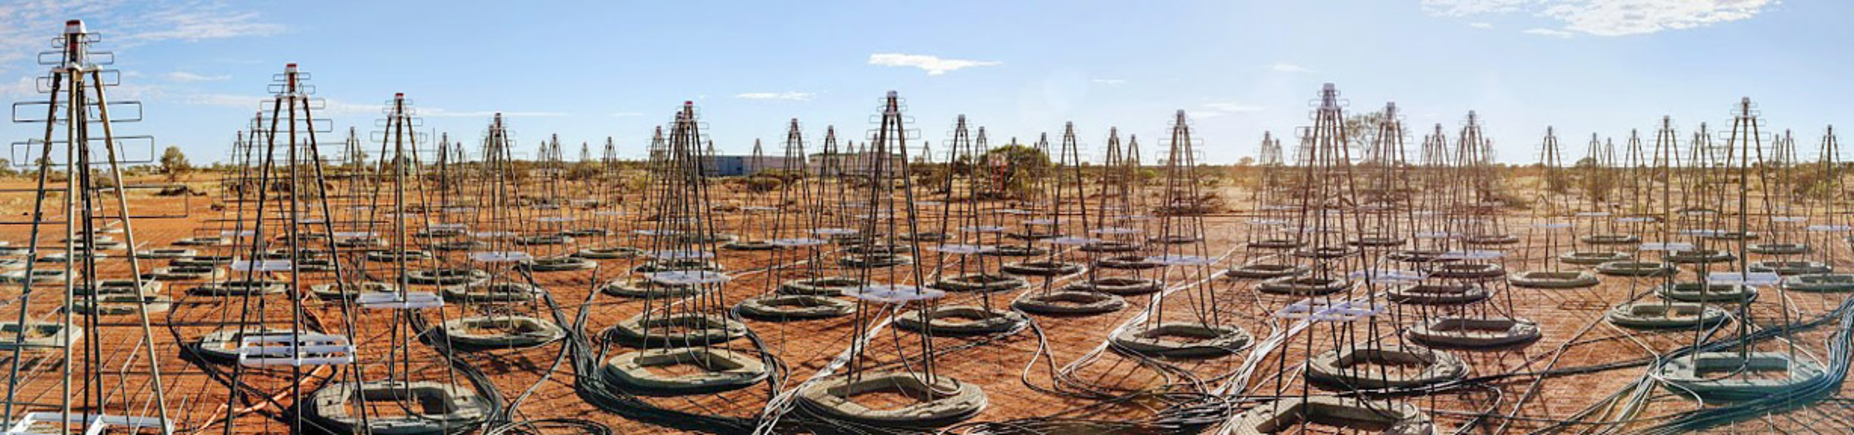
\includegraphics[width=\columnwidth]{FRAPL01f4}
  \caption{SKA1-Low prototype antenna station as deployed in the MRO.}
  \label{fig:SKA1-Low_prototype_station}
\end{figure}


The interested reader can follow \cite{SKA-TEL-SKO-0000002_03}, that defines the baseline design capabilities of both the SKA1-Mid and SKA1-Low telescopes.


% section ska1_telescopes (end)

\section{SKA1 Pre-Construction} % (fold)
\label{sec:ska1_preconstruction}

Both SKA1-Mid and SKA1-Low are being design by 9 international design consortia, which have each taken over 9 major high-level work packages that make up the work required to deliver the designs for those two telescopes:

\begin{itemize}
	\item[DSH] Dish Consortium, led by the Commonwealth Scientific and Industrial Research Organization (CSIRO; Australia); responsible for the design of the SKA1-Mid dishes, including their receivers, internal control system, and the delivery of tested SKA1-Dish prototypes;
	\item[LFAA] Low-Frequency Aperture Array, led by ASTRON (Netherlands); responsible for the design of the SKA1-Low antennas and station-level beamforming and calibration systems, and the delivery of tested SKA1-Low antenna and station prototypes;
	\item[SADT] Synchronisation and Data Transport, led by University of Manchester (UK); responsible for the design of the networks that interconnect Dishes (in SKA1-Mid) or Stations (in SKA1-Low) with the correlators, and the beamformed data and calibrated visibility data from the correlator/beamformer to the science data processing sub-system; it also includes the frequency and time reference system, and the UTC(SKA) implementation;
	\item[TM] Telescope Manager, led by National Centre for Radio Astrophysics (NCRA; India); responsible for the design of the control and monitoring system of the telescope, and the observation management, from proposal handling, to planning, to live scheduling;
	\item[CSP] Central Signal Processor, led by the National Research Council of Canada (NRC); responsible for the design of the SKA1-Mid and SKA1-Low correlator/beamformer, and also the PulSar Search (PSS) and PulSar Timing (PST) beam-data processing engines;
	\item[SDP] Science Data Processor, led by University of Cambridge (UK); responsible for the design of the science processing of calibrated visibilities, transient data, tied-array beams, and beam-formed time-series data;
	\item[INAU] Infrastructure Australia, led by the Commonwealth Scientific and Industrial Research Organization (CSIRO; Australia); responsible for the design of all supporting infrastructure of the SKA1-Low telescope, except for networking and telephony services;
	\item[INSA] Infrastructure South Africa, led by SKA~SA (South Africa); responsible for the design of all supporting infrastructure of the SKA1-Mid telescope, except for networking and telephony services, and of the site buildings, which are provided as part of the South African hosting agreement;
	\item[AIV] Assembly, Integration, and Verification, led by SKA~SA (South Africa); responsible for the construction roll-out plan and the verification, validation, and integration plans for the SKA1-telescopes.
\end{itemize}

There are three additional international consortia working on technologies that will not be used for the SKA1 telescopes, but will be part of either in future upgrades, or for SKA2 telescopes, as part of what is known as the Advanced Instrumentation Program (AIP):

\begin{itemize}
	\item[MFAA] Medium-Frequency Aperture Array, led by ASTRON (Netherlands); responsible for developing prototypes and de-risking aperture array technologies at medium frequencies (above 450 MHz);
	\item[PAF] Phased-Array Feed, led by the Commonwealth Scientific and Industrial Research Organization (CSIRO; Australia); includes improvements to the Phased-Array Feed (PAF) technology being developed for the ASKAP precursor telescope;
	\item[WBSPF] Wide-Band Single Pixel Feed, led by Chalmers University (Sweden); responsible for the design of broad-spectrum, single-pixel feed receivers, that go beyond 4:1 bandwidth ratios;
\end{itemize}

These consortia are not directly funded by the SKA Organisation, but instead the organisations making up those consortia get their funding through funding programs created by the member countries of the SKA, or by non-SKA-specific  funding instruments from countries not yet members of the SKA. This is specific for the Pre-Construction phase.

The framework for funding the construction is being negotiated together with the IGO Convention, but it will most likely consist of a mixture of cash and in-kind contributions to the future SKA IGO, with measures to attempt a \emph{juste retour} to member countries.

The Convention will be initialised in October 2017, with Convention Signing by the representatives of the members in January 2017. After that, a ratification process in each member country is required.

The SKA IGO Convention will enter into force when at least 5 member countries, with the 3 host countries (Australia, South Africa, and United Kingdom) among them, have ratified the Convention. After that date, there will be a period of coexistence between the SKA IGO and the SKA Organisation, and a take over process of the SKA Organisation assets by the SKA IGO will take place during the Transition period.

Meanwhile, the Pre-Construction engineering process will end up with Critical Design Review (CDR) process for all design workpackages, and a following System CDR. When the CDR process is closed out, a Construction Proposal will be created to be ready for the moment in which the SKA IGO Council exists. Acceptance of the proposal is expected around Q3 2019, with construction ramping up after that.

The timeline for the above mentioned events is shown in Fig.~\ref{fig:IntegratedTimeline_v5}.
 
\label{sec:ska1_timeline}
 \begin{figure*}[!tb]
   \centering
     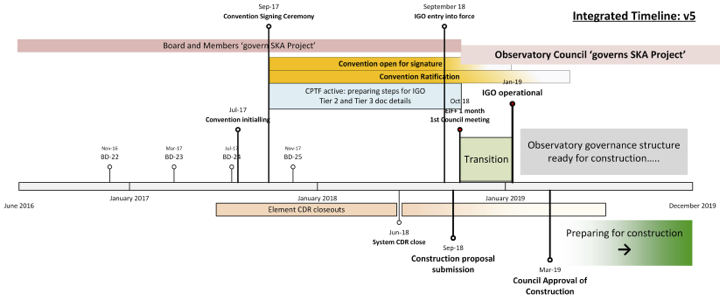
\includegraphics[width=\textwidth]{FRAPL01f5}
   \caption{Integrated SKA1 timeline, showing organisation governance, engineering design, and funding tracks up to construction.}
   \label{fig:IntegratedTimeline_v5}
 \end{figure*}
 

% section sec:ska1_preconstruction (end)

\section{SKA1 Data Flow \& Processing} % (fold)
\label{sec:ska1_data_flow_and_processing}

One of the main challenges that the SKA1 telescopes pose is the need for almost real-time processing —for the calibration loops— of tens of terabits of information. A notional data flow for the SKA1-Mid and SKA1-Low telescopes is shown in Fig.~\ref{fig:SKA1_NotionalDataFlow}.

For SKA1-Mid, the 133 SKA1 Dishes, together with the 64 MeerKAT dishes, generate a traffic of up to 8.8 terabit/second to the SKA1-Mid Correlator (part of the Central Signal Processor, CSP).

For SKA1-Low, the aggregate data traffic from the antennas is up to 2 petabit/second, and is further reduced by the LFAA beamformer down to 7.2 terabit/second, which is then fed to the SKA1-Low correlator (CSP).

For comparison, CISCO estimates that in 2016 the average data across all of the internet was 360 terabit/s, or $1/5$ of the traffic generated by the SKA1-Low antennas, and only ~40 times the traffic generated by all the SKA1-Mid antennas.

At the CSP the main operations are Multipy-ACcumulate operations (MACs), and the computational intensity required is of around 50 petaflops\footnote{$50 \times 10^{15}$ FLoating-point OPerations per Second} to generate radio interferometric visibility data, which is then sent to the Science Data Processor through a data link of ~5 terabit/second.

The SDP for both SKA1-Mid and SKA1-Low will be formed by a High-Performance Computer in the order of 250 petaflops\footnote{$250\times10^{15}$ FLoating-point OPerations per Second}, and the amount of science data that will be archived is estimate in the order of 300 petabyte/year. 

\begin{figure}[!tb]
  \centering
    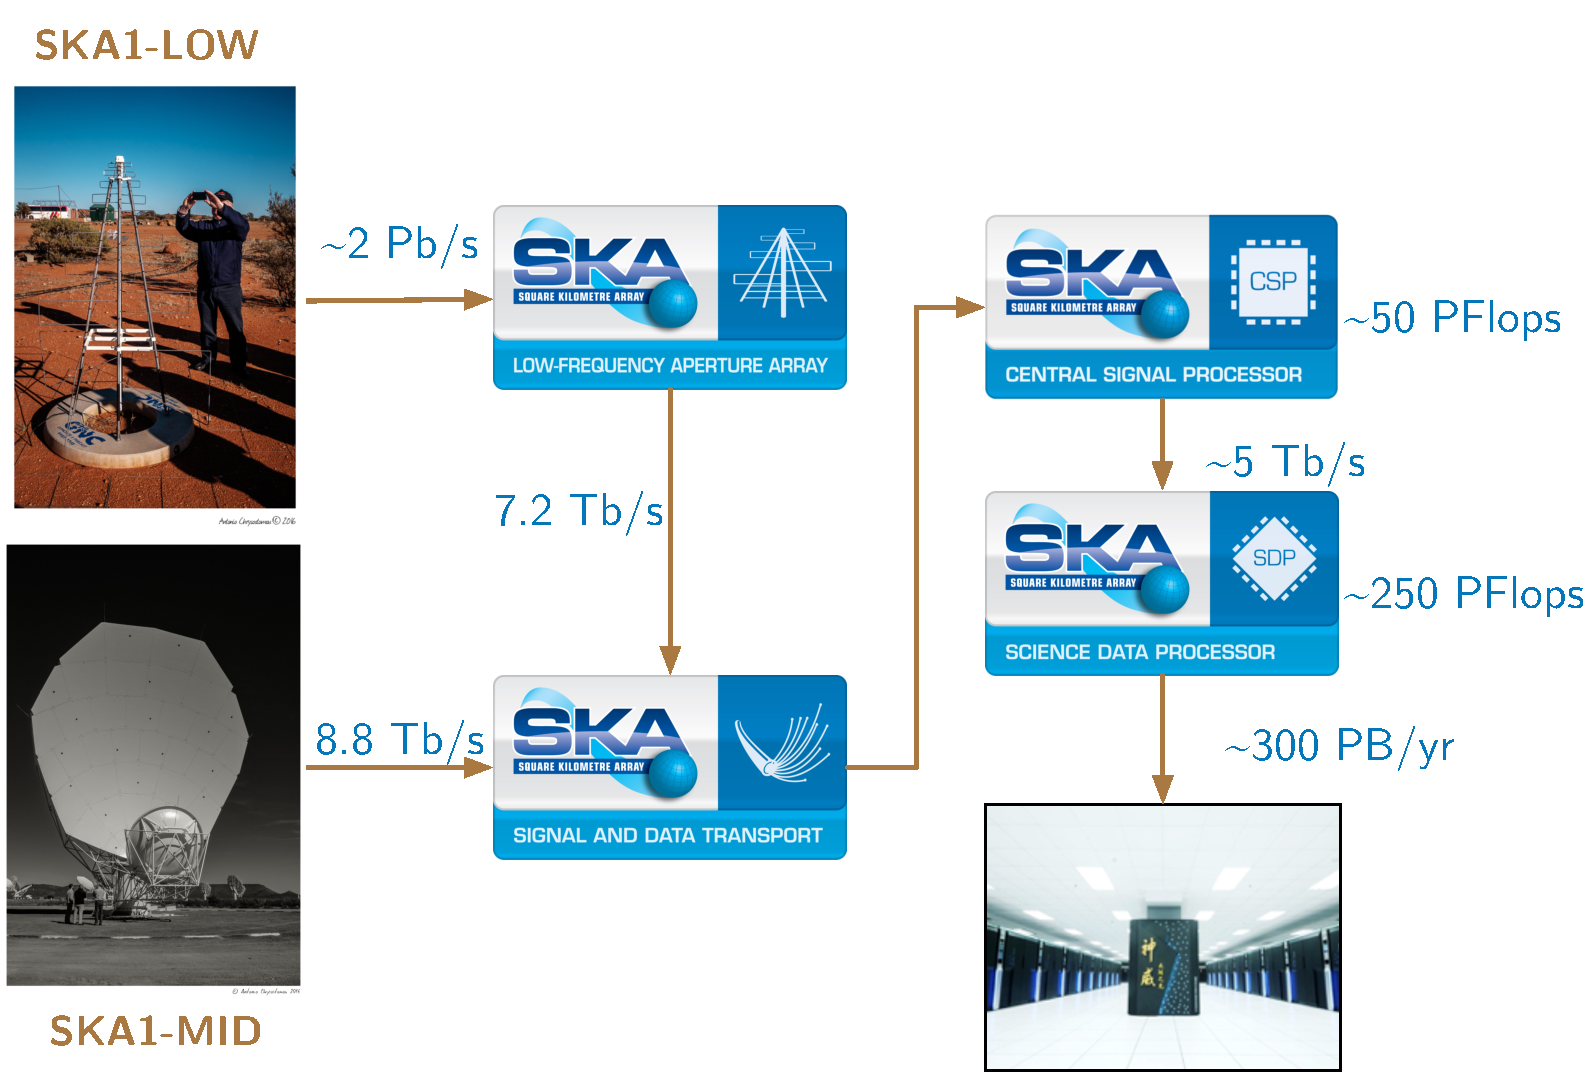
\includegraphics[width=\columnwidth]{FRAPL01f6}
  \caption{Notional data flows and computational intensity required by the SKA1 telescopes, with shared Central Signal Processor (CSP) and Science Data Processor (SDP) for convenience.}
  \label{fig:SKA1_NotionalDataFlow}
\end{figure}

The large amount of data to be archived, and the large size of the individual observations that researchers will have to analyse makes it very difficult to distribute the data directly to the investigatores. A network of SKA Regional Centres (SRCs) is being envisioned to share the storage of the SKA1 telescopes' archives, and provide data access to the investigators and archive researchers, but also scientific analysis tools, and custom pipelines for dedicated science goals.	

The different SRCs will be federated in an SKA Regional Centre Alliance (SRCA) that will provide a unified front-end for astronomers. Fig.~\ref{fig:SRCs} illustrates the concept.

\begin{figure}[!tb]
  \centering
    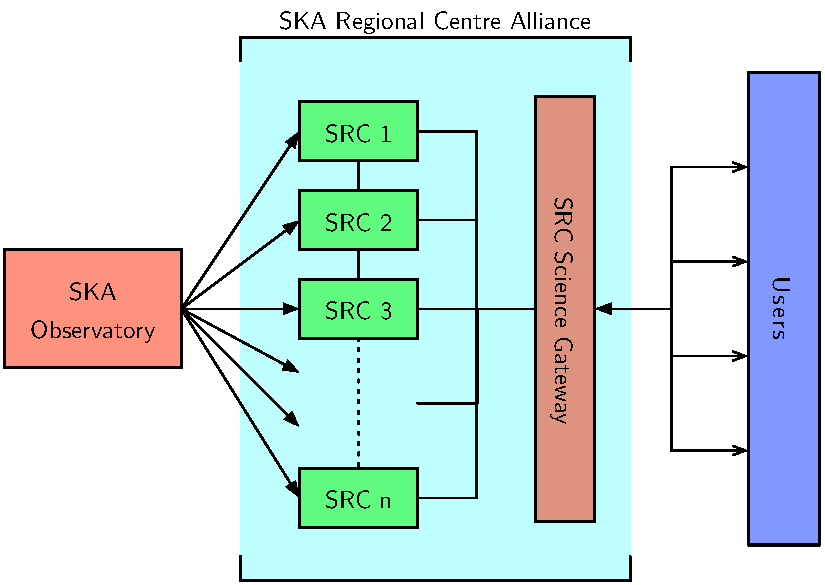
\includegraphics[width=\columnwidth]{FRAPL01f7}
  \caption{The SKA Regional Centre Alliance is composed of a number of SKA Regional Centres, that will store the data from the SKA telescopes, and will provide a unified access and processing gateway to investigators.}
  \label{fig:SRCs}
\end{figure}

The fastest supercomputer in the TOP500 list as of June 2017\footnote{https://www.top500.org/lists/2017/06/} is the Sunway TaihuLight, developed by China’s National Research Center of Parallel Computer Engineering and Technology (NRCPC), with a Linpack performance of 93 petaflops. Each of the SKA1 SDPs will have to be, then, 5 times more powerful than the current fastest computer in the world.

Given the challenge to achieve that performance, and the experience that CERN has in high-perfomance computing and its tiered network of data and computing centres for the analysis of the data coming from the Large Hadron Collider (LHC) experiments, CERN and SKA have signed an agreement for collaboration on extreme-scale computing\footnote{http://skatelescope.org/news/ska-signs-big-data-cooperation-agreement-cern/}.

% section ska1_data_flow_and_processing (end)

\section{SKA1 Software, Control System Guidelines, and Processes} % (fold)
\label{sec:ska1_software_control_system_guidelines_SAFe}

The SKA1 telescopes will be composed of millions of parts that will be controlled, monitored, and orchestrated by the subsystem called Telescope Manager. 

It was envisioned that the Telescope Manager (TM) would be the top of a control hierarchy at telescope level, while each SKA subsystem had a Local Monitoring and Control (LMC) unit that translated high-level coordination commands into domain-specific instructions, and reported rolled-up status information to TM. The LMCs had to support additional drill-down and pass-through capabilities when requested.

In March 2015 it was decided that the Telescope Manager middleware should be an existing, open source, industrial strength Supervisory Control And Data Acquisition system.

After analysing the ALMA Control Software (ACS)\footnote{https://github.com/ACS-Community/ACS/}, the Experimental Physics and Industrial Control System (EPICS)\footnote{Experimental Physics and 
Industrial Control System}, and the TACO Next Generation Object-oriented control system (TANGO)\footnote{http://www.tango-controls.org/}, TANGO was selected as the middleware of choice for the SKA telescopes.

In order to avoid problems with the interpretation of TANGO patterns, a series of meetings were arranged so that the developers of the LMCs for the different SKA subsystems (also known as Elements in SKA parlance) had common approaches, and common ways of reporting state and health information, and the ways in which pass-through and drill-down capabilities were mapped to the TANGO framework.

The result was a series of technical notes, and three main documents applicable to control interfaces: the SKA Control System Guidelines, the SKA TANGO Developer Guidelines, and the SKA TANGO Naming Convention. You can read more about them in~\cite{ICALEPCS17-MOBPL03}.

\begin{figure*}[!tb]
  \centering
    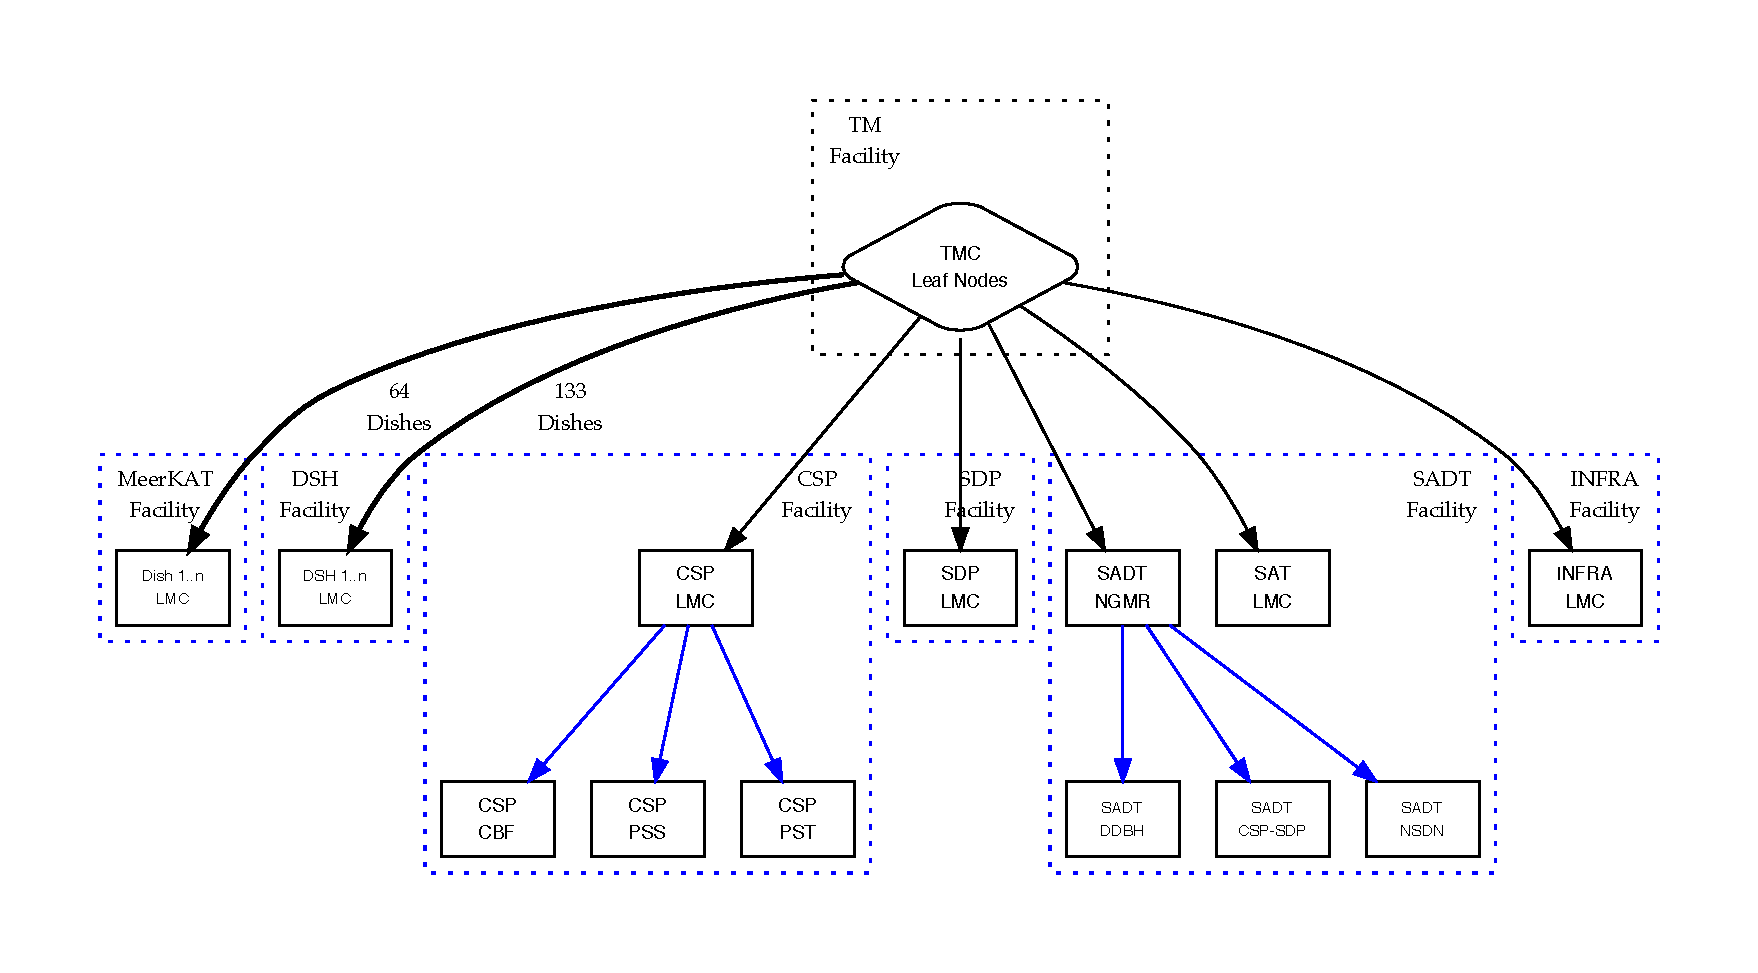
\includegraphics[width=.95\textwidth]{FRAPL01f8}
  \caption{High-level overview of the SKA1-Mid Facilities. There are 133 Facilities for each of the SKA1-Mid dishes, while there is only one facility for the 64 MeerKAT dishes. Compare with Fig.~\ref{fig:ControlHierarchyLow}.}
  \label{fig:ControlHierarchyMid}
\end{figure*}

\begin{figure*}[!tb]
  \centering
    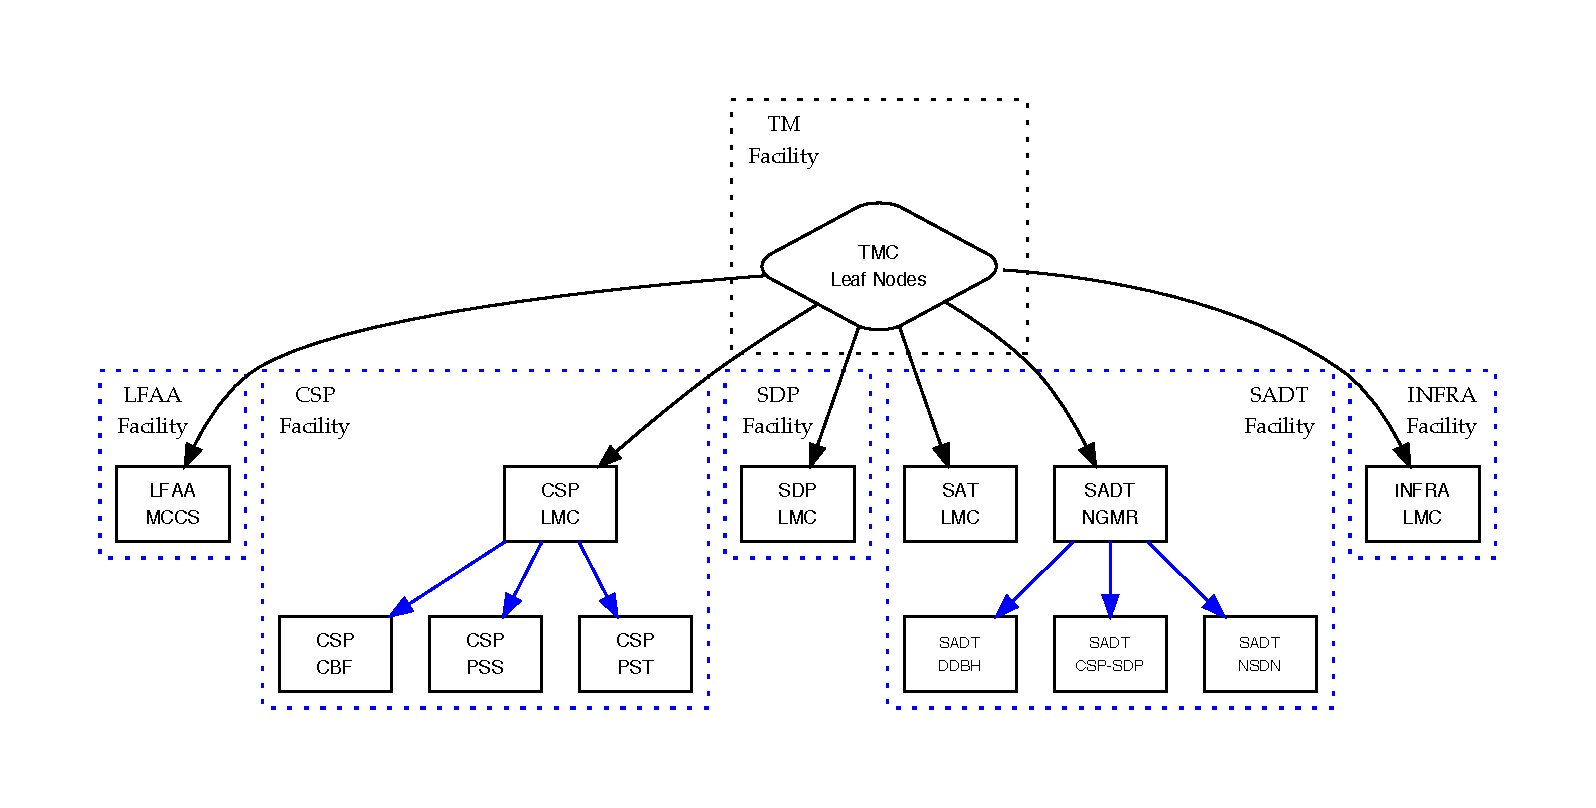
\includegraphics[width=.95\textwidth]{FRAPL01f9}
  \caption{High-level overview of the SKA1-Low Facilities. The LFAA MCCS exposes control to a very large hierarchy of devices, not shown here. Compare with Fig.~\ref{fig:ControlHierarchyMid}.}
  \label{fig:ControlHierarchyLow}
\end{figure*}

The high-control hierarchy for SKA1-Mid is shown in Fig.~\ref{fig:ControlHierarchyMid}, while the one for SKA1-Low is shown in Fig.~\ref{fig:ControlHierarchyMid}.

The diagrams show that there is a TANGO facility for each of the SKA elements, except in the case of Dish, where a facility for each of the individual dishes is foreseen. This helps each dish to be really identical from a control point of view, and to keep their device hierarchies separate from each other.

In the case of SKA1-Low, below the MCCS a number of TANGO devices will exist to monitor equipment at least down to tile level (SKA1-Low stations are made up of 16 tiles, or 16 antennas each), which means at least 8,192 devices.

The SDP is primarily a High-Performance Computer, and as such tools such as Open Stack will be used for monitoring and orchestrating the software processes that need to be launched as a result of observation processing, and a graph execution engine (the SDP Execution Framework), based on Apache Hadoop and/or Apache Spark, and orchestrated by Apache Mesos or Apache Marathon will be used, insted of using TANGO directly for orchestration of those processes. However, pools of ProcessBlocks TANGO devices will be created that will help to provide observation progress monitoring through TANGO.

The complexity of a system that will encompass, when developed, several millions lines of code, induces both programmatic and functional risk. In order to avoid that, the SKAO has recently decided to adopt the Scaled Agile Framework\footnote{http://www.scaledagileframework.com} (SAFe\textregistered).

We have started processes to make the core concepts of Agile in general, and SAFe in particular, an integral part of the software development plans of the SKA consortia. The balance between the traditional strict, gated System Engineering approaches of large construction projects, and the agile principles for continuous integration and delivery of software is not trivial to achieve, and will be the focus of the SKAO for the future, together with the successful completion of the subsystem- and system-level CDRs.

Figure~\ref{fig:FRAPL01f10} shows the SAFe processes for software engineering. The bottom part of it represents the work of a single Agile team, while the middle part represents the Agile Solution Train (ART) that combines the work of several Agile teams, and the top part represents the Solution Train, that combines several ARTs.

\label{sec:scaled_agile_framework}
\begin{figure*}[!tb]
  \centering
    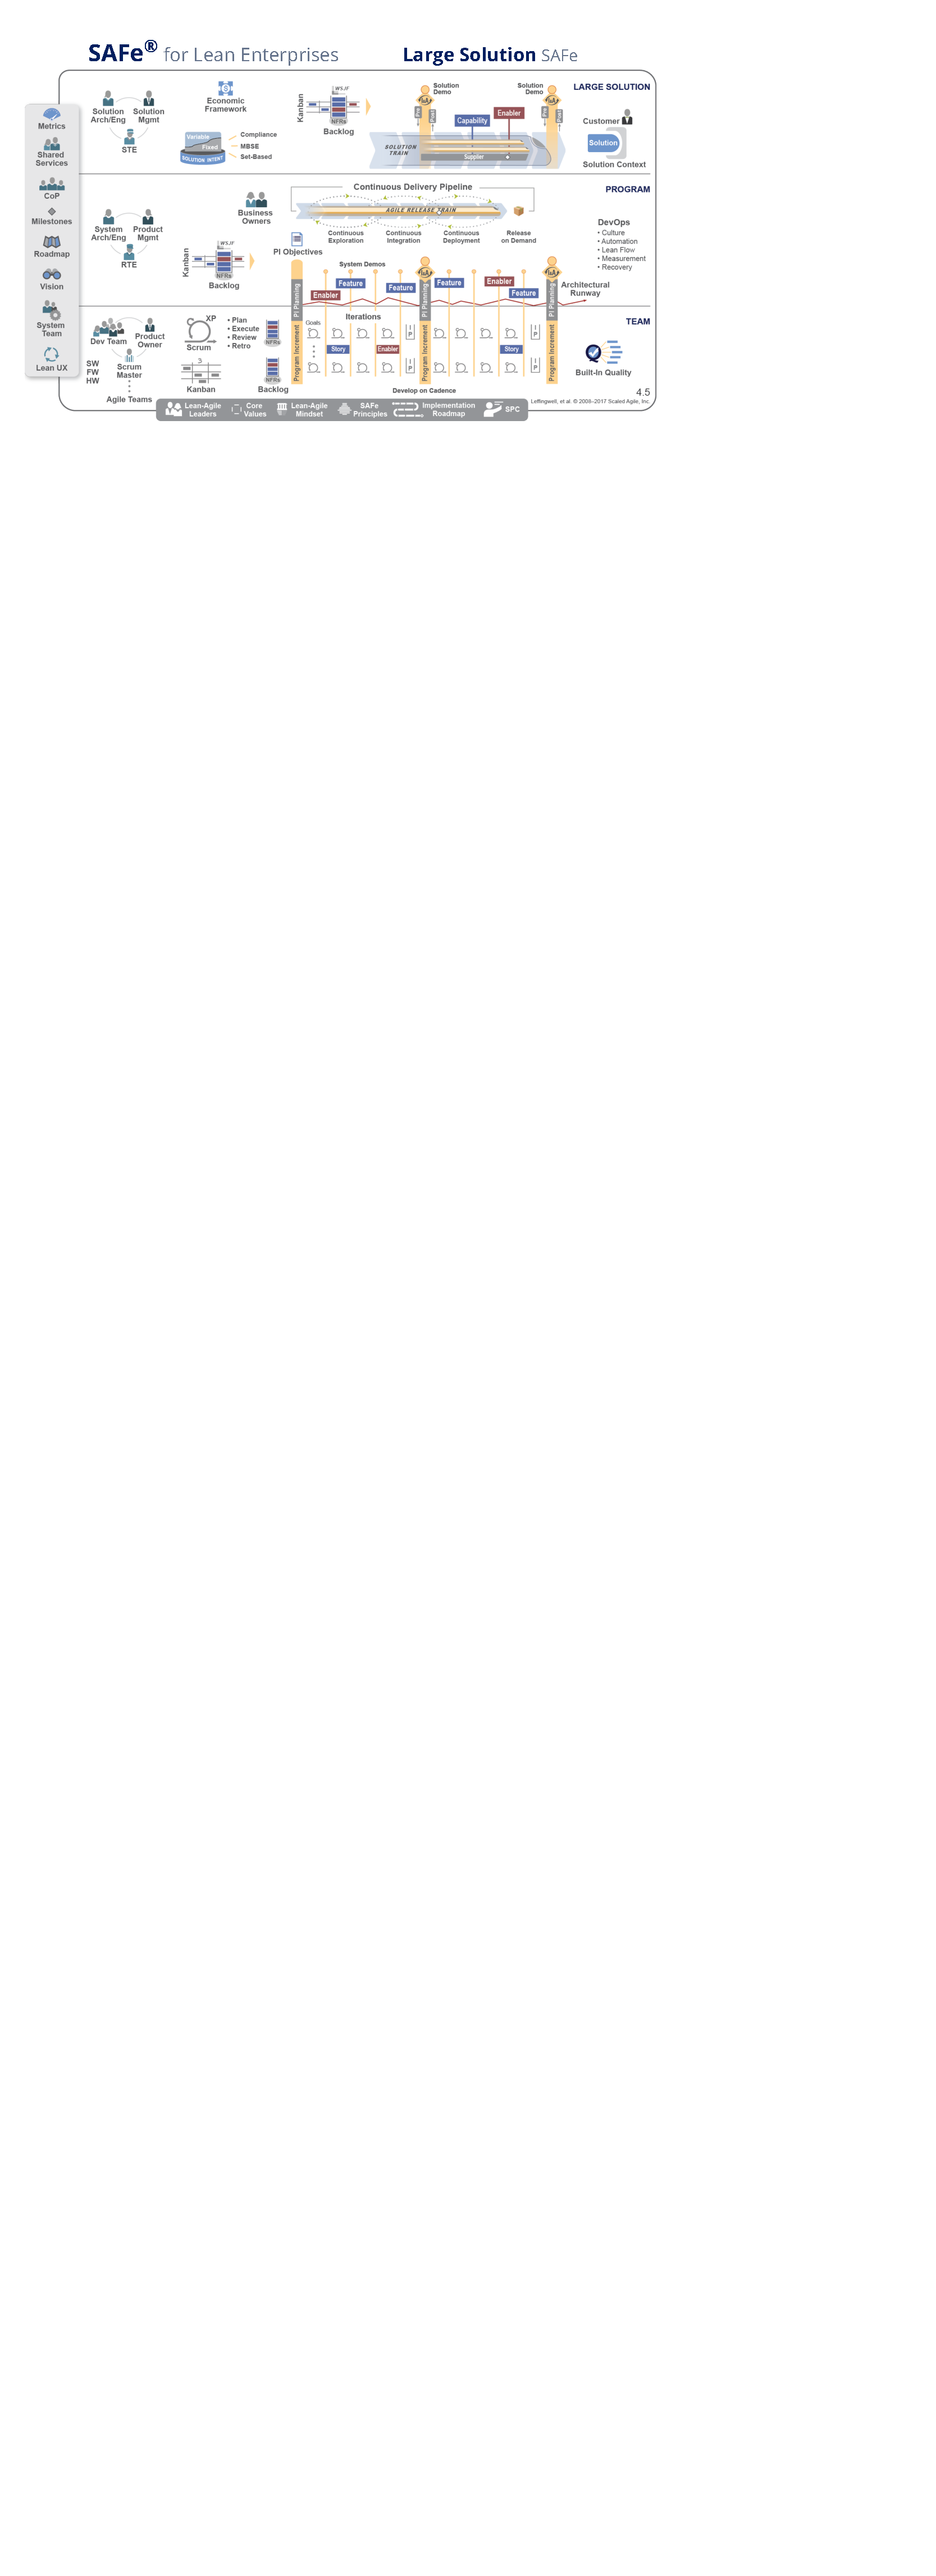
\includegraphics[width=\textwidth]{FRAPL01f10.pdf}
  \caption{Diagram of Scaled Agile Framework (SAFe\textregistered) processes for software engineering.}
  \label{fig:FRAPL01f10}
\end{figure*}

The main tool for synchronising the processes of the Agile Release Trains, and the individual agile teams is the cadence of the sprints and Program Increments (PIs), and the sharing of a common backlog that the teams self-organise every Program Increment, so that work dependencies, and programme/solution needs are resolved at every Program Increment. Feedback from the solution intent is flown down from Model Based System Engineering artifacts at the top, to the backlogs for the ARTs, and the individual teams, with always a representation of that solution intent in the form of Product Owners, System Engineers, and Solution Architects.

We're in the process of deriving what the first PIs will be from the current AIV roll-out plan, so that we can provide the functionality that is required precisely when it is needed.

% section ska1_control_hierarchy_and_control_system_guidelines (end)


\section{Conclusion} % (fold)
\label{sec:conclusion}
The SKA1 telescopes are just a few months from their Critical Design Reviews, and that of their subsystems, and their construction will prove challenging both in terms of organisational readiness, and the complexity of the systems being built.

As part of the derisking of the software systems, and managing that complexity, we have opted for several standard solutions:

\begin{itemize}
	\item using a horizontal harmonisation approach to control systems, choosing TANGO as the control framework and middleware for all subsystems of the SKA1 telescopes; TANGO provides the right level of hierarchical control and encapsulation, and easy access to all parts of the control system, combined with a rich software library and a vibrant community;
	\item using an industry supported agile process framework such as SAFe to successfully scale agile practices to a large scale solution, with continuous integration at team and solution levels;
\end{itemize}

We expect to be able to have a construction proposal and an IGO in Q1 2019, and to start procurement in late 2019, with the first antennas on the ground around late 2022, and a complete deployment in 2026, with the ramp to operations starting soon after that.

% section conclusion (end)

\section{Acknowledgement} % (fold)
\label{sec:acknowledgement}
The authors want to thank all colleagues at the SKA Organisation for useful discussions that have helped in clarifying the different aspects of all SKA subsystems. The authors would also like to thank all the participants in the LMC Harmonisation meetings, and to the members of the ANT\footnote{Because ants can support loads many times their weight, something that tigers can't do…} team that wrote the SKA Control System Guidelines and supporting technical notes.

% section acknowledgement (end)

%\section*{References} % (fold)
\label{sec:references}
\printbibliography

% section references (end)




\end{document}
